\documentclass[aspectratio=169,11pt]{beamer}
\usepackage[T1]{fontenc}
\usepackage[utf8]{inputenc}
\usepackage{lmodern,amsmath,amssymb,graphicx,tikz}
\usetikzlibrary{arrows.meta,calc}
\usetheme{default}
\usefonttheme{serif}
\setbeamercolor{normal text}{fg=black,bg=white}
\setbeamercolor{structure}{fg=black}
\setbeamercolor{frametitle}{fg=black}
\setbeamercolor{title}{fg=black}
\setbeamertemplate{navigation symbols}{}
\setbeamertemplate{footline}[frame number]
\setbeamertemplate{itemize items}[circle]
\setbeamersize{text margin left=8mm,text margin right=8mm}
\setlength{\parskip}{5pt}
\newcommand{\cO}{\mathcal O}
\newcommand{\cI}{\mathcal I}
\newcommand{\cA}{\mathcal A}
\newcommand{\db}{\bar\partial}
\newcommand{\C}{\mathbb C}
\newcommand{\Pj}{\mathbb P}
\newcommand{\norm}[1]{\lVert#1\rVert}
\newcommand{\src}[1]{\par\vfill{\scriptsize #1\par}}
\author{Daniel Gonz\'alez Casanova Azuela}

\title{Kodaira embedding through vanishing}
\subtitle{Lecture 23: the mechanism and Nadel's theorem}
\date{Hodge theory}
\begin{document}
\begin{frame}\titlepage\end{frame}
\begin{frame}{The course so far}
\begin{enumerate}
\setlength{\itemsep}{12pt}
\item \textbf{Complex structures and holomorphic functions.}\\
\(I^2=-1\), Cauchy's formula, and complex manifolds.
\item \textbf{Integrability.}\\
Frobenius, real analytic methods, and Newlander--Nirenberg.
\item \textbf{Kähler geometry.}\\
Homogeneous examples and Fubini--Study; Levi-Civita, intrinsic torsion, and Bismut.
\end{enumerate}
\end{frame}

\begin{frame}{The course so far (continued)}
\begin{enumerate}
\setcounter{enumi}{3}
\setlength{\itemsep}{9pt}
\item \textbf{Hodge theory and Kähler identities:} harmonic representatives.
\item \textbf{Sheaves and Dolbeault:} cohomology through the \(\db\)-complex.
\item \textbf{Chern curvature and bundle-valued Hodge theory:}\\
Bochner--Kodaira and Kodaira--Nakano vanishing.
\item \textbf{The analytic extension:} Hilbert-space operators and \(L^2\);
holomorphic convexity, Stein spaces, and pseudoconvex vanishing;
currents, singular psh weights, and Poincaré--Lelong.
\end{enumerate}
\end{frame}

\begin{frame}{Projective space has a positive form}
\(\Pj^n\) is the set of lines through the origin in \(\C^{n+1}\); \(\pi\) sends a nonzero vector to its line.
\par\medskip
On nonzero vectors \(Z\in\C^{n+1}\), define
\[
\tilde\omega=\frac{i}{2\pi}\,\partial\db\log|Z|^2,\qquad |Z|^2=|Z_0|^2+\cdots+|Z_n|^2.
\]
It is \textbf{basic}: for every vector field \(V\) along the fibres of \(\pi\),
\[
\iota_V\tilde\omega=0,\qquad \mathcal L_V\tilde\omega=0.
\]
So it comes from a form downstairs, the \textbf{Fubini--Study form}: \(\tilde\omega=\pi^*\omega_{\rm FS}\).
\src{Fubini (1904), Study (1905). Scaling \(Z\mapsto\lambda Z\) adds \(\log|\lambda|^2\), which \(\partial\db\) kills.}
\end{frame}

\begin{frame}{The Fubini--Study form is positive}
Upstairs, on \(v\in\C^{n+1}\) and up to a positive factor, \(\tilde\omega\) gives
\[
\frac{|Z|^2|v|^2-|\langle v,Z\rangle|^2}{|Z|^4}\ \ge\ 0 .
\]
By Cauchy--Schwarz, equality holds exactly when \(v\in\C Z\): the direction of the fibre.
\par\medskip
Since \(d\pi_Z\) is onto \(T_{[Z]}\Pj^n\) with kernel \(\C Z\),
\[
\boxed{\omega_{\rm FS}\ \text{is positive on every nonzero tangent vector of}\ \Pj^n.}
\]
\end{frame}

\begin{frame}{Positivity passes to submanifolds}
Let \(X\subset\Pj^N\) be a compact complex submanifold.
\par\bigskip
Restrict the line bundle: \(L=\cO(1)|_X\).
\par\medskip
Its curvature is \(\omega_{\rm FS}|_X\), and it is still positive.
\par\bigskip
\begin{center}
\Large\(X\) projective \(\ \Longrightarrow\ \) \(X\) has a positive line bundle.
\end{center}
\par\bigskip
Question: is the converse true?
\end{frame}

\begin{frame}{The goal of both lectures: Kodaira embedding}
Let \(X\) be compact complex and \(L\) a holomorphic line bundle with a smooth positive metric.
For all sufficiently large \(N\),
\[
\boxed{\Phi_{L^N}:X\hookrightarrow
\Pj\bigl(H^0(X,L^N)^*\bigr)}
\]
is a holomorphic embedding.
\end{frame}

\begin{frame}{Kunihiko Kodaira (1915--1997)}
\begin{columns}[c]
\column{.36\textwidth}
\centering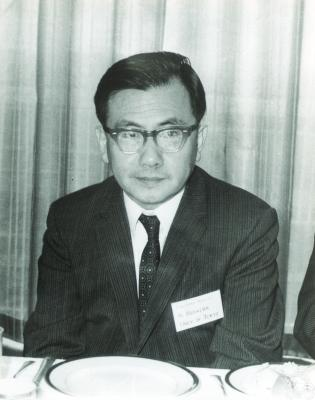
\includegraphics[height=4.8cm]{../assets/Kunihiko_Kodaira.png}
\column{.59\textwidth}
Fields Medal, 1954.
\par\bigskip
His idea: an \textbf{analytic} condition (curvature)
produces an \textbf{algebraic} object (polynomial equations).
\end{columns}
\src{Photo: Konrad Jacobs / MFO, Tokyo 1969, CC BY-SA 2.0 DE. Historical source: IAS scholar profile.}
\end{frame}

\begin{frame}{Where this sits in history}
\begin{center}
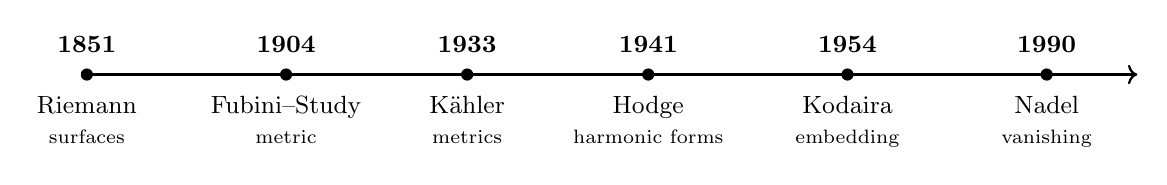
\begin{tikzpicture}[x=1.15cm]
\draw[thick,->] (0,0)--(11.6,0);
\foreach \x/\y/\t/\s in {
 0/1851/Riemann/surfaces,
 2.2/1904/Fubini--Study/metric,
 4.2/1933/Kähler/metrics,
 6.2/1941/Hodge/harmonic forms,
 8.4/1954/Kodaira/embedding,
 10.6/1990/Nadel/vanishing}
{\fill (\x,0) circle (2.2pt);
 \node[above] at (\x,.15) {\small\textbf{\y}};
 \node[below,align=center] at (\x,-.15) {\small \t\\[-1pt]\scriptsize\s};}
\end{tikzpicture}
\end{center}
\par\bigskip
One theme: \textbf{analysis proves that enough holomorphic functions exist}.
\par\medskip
Riemann used analysis to prove that compact Riemann surfaces are algebraic curves.
Kodaira did the same in every dimension.
\end{frame}

\begin{frame}{An embedding needs values and derivatives}
\[
\begin{array}{r@{\;}c@{\;}c@{\;}l}
\Phi_{L^N}\colon & X & \longrightarrow & \Pj\bigl(H^0(X,L^N)^*\bigr)\\
& x & \longmapsto & [s_0(x):\cdots:s_M(x)]
\end{array}
\qquad s_0,\ldots,s_M \text{ a basis of } H^0(X,L^N).
\]
\begin{center}
\renewcommand{\arraystretch}{1.8}
\begin{tabular}{ll}
\(\Phi_{L^N}\) is & Language of sections\\
\hline
Defined everywhere & \textbf{Base-point free}: no common zero\\
Injective & \textbf{Separates points}: independent values\\
An immersion & \textbf{Separates tangent directions}
\end{tabular}
\end{center}
\end{frame}

\begin{frame}{Vanishing lifts prescribed data}
Put \(A=L^N\). For an ideal sheaf \(I\),
\[
0\longrightarrow A\otimes I\longrightarrow A
\longrightarrow A\otimes(\cO_X/I)\longrightarrow0.
\]
The long exact sequence contains
\[
H^0(X,A)\longrightarrow H^0(X,A\otimes\cO_X/I)
\longrightarrow H^1(X,A\otimes I).
\]
\[
\boxed{H^1(X,A\otimes I)=0
\quad\Longrightarrow\quad\text{every prescribed quotient section lifts}.}
\]
\end{frame}

\begin{frame}{The task is a vanishing theorem}
We want, for one sufficiently large \(N\),
\(H^1(X,L^N\otimes I)=0\) for three ideals:
\begin{center}
\renewcommand{\arraystretch}{1.6}
\begin{tabular}{lll}
\(I=\mathfrak m_x\) & gives & base-point freeness\\
\(I=\mathfrak m_x\cap\mathfrak m_y\) & gives & point separation\\
\(I=\mathfrak m_x^2\) & gives & tangent separation
\end{tabular}
\end{center}
Kodaira vanishing handles a positive bundle with a canonical twist.
We need a theorem that also allows these ideals.
\end{frame}

\begin{frame}{Reminder: the Chern connection}
For a Hermitian holomorphic line bundle \((L,h)\),
\[
\nabla:C^\infty(X,L)\longrightarrow\Omega^1(X,L),\qquad
\nabla(fs)=df\otimes s+f\nabla s.
\]
It preserves \(h\), and its \((0,1)\)-part is \(\db_L\).
\par\medskip
In a holomorphic frame \(e\), with \(|e|_h^2=h(e,e)\),
\[
\nabla(fe)=\bigl(df+f\,\partial\log|e|_h^2\bigr)\,e.
\]
On bundle-valued forms, \(\nabla=d+\partial\log|e|_h^2\wedge\), by the graded Leibniz rule.
\end{frame}

\begin{frame}{Reminder: curvature and its class}
Squaring the connection gives multiplication by a two-form:
\[
\nabla^2=\Theta_h\wedge,\qquad
\Theta_h=d\bigl(\partial\log|e|_h^2\bigr)=-\partial\db\log|e|_h^2.
\]
\begin{itemize}
\setlength{\itemsep}{8pt}
\item \(d\Theta_h=0\): locally it is exact, \(d\bigl(\partial\log|e|_h^2\bigr)\).
\item \(\Theta_h\) is imaginary-valued and of type \((1,1)\); \(i\Theta_h\) is real.
\item \(\displaystyle c_1(L)_{\mathbb R}=\left[\frac{i}{2\pi}\Theta_h\right]\):
its periods on integral two-cycles are integers.
\end{itemize}
\medskip
For a vector bundle \(E\), curvature is endomorphism-valued; take the trace:
\(\displaystyle c_1(E)_{\mathbb R}=\left[\frac{i}{2\pi}\operatorname{tr}\Theta_E\right]\).
\end{frame}

\begin{frame}{Reminder: what positivity means}
A real \((1,1)\)-form \(\alpha\) gives a symmetric form
\[
g_\alpha(v,w)=\alpha(v,Iw),\qquad v,w\in T_xX.
\]
It is \textbf{positive} if \(\alpha(v,Iv)>0\) for every \(v\ne0\).\\
Replacing \(>0\) by \(\ge0\) gives \textbf{semipositivity}.
\par\bigskip
A holomorphic line bundle is \textbf{positive} if it admits a smooth metric with
\[
\boxed{i\Theta_h>0.}
\]
We test tangent vectors to \(X\), not vectors in the fibre of \(L\).
\end{frame}

\begin{frame}{Fubini--Study is the curvature of \(\cO(1)\)}
The fibre of \(\cO(1)\) at \([Z]\) is the dual of the line \(\C Z\).
Measure the line with the norm of \(\C^{n+1}\).
\par\medskip
The coordinate \(Z_0\) is a holomorphic frame where \(Z_0\ne0\), with
\[
|Z_0|_h^2=\frac{|Z_0|^2}{|Z|^2}.
\]
Pulled back to \(\C^{n+1}\setminus\{0\}\), since \(\partial\db\log|Z_0|^2=0\),
\[
\Theta_h=-\partial\db\log|Z_0|_h^2=\partial\db\log|Z|^2,
\qquad\text{so}\qquad
\boxed{\tfrac{i}{2\pi}\Theta_h=\omega_{\rm FS}.}
\]
Thus \(\cO(1)\) is positive.
\end{frame}

\begin{frame}{Nadel vanishing}
Let \((X,\omega)\) be compact Kähler of dimension \(n\), and \(B\) a holomorphic line bundle.
A singular metric \(h\) with
\[
i\Theta_h\ge\varepsilon\omega,\qquad \varepsilon>0,
\]
gives
\[
\boxed{H^q(X,K_X\otimes B\otimes\cI_h)=0\quad(q>0).}
\]
The new object is the multiplier ideal \(\cI_h\).
\end{frame}

\begin{frame}{Alan Michael Nadel}
\begin{columns}[c]
\column{.44\textwidth}
\centering

\begin{tikzpicture}
\fill[black!12] (.12,-.12) rectangle (4.32,5.08);
\filldraw[fill=blue!4,draw=blue!50!black] (0,0) rectangle (4.2,5.2);
\draw[blue!50!black,line width=2pt] (.2,0)--(.2,5.2);
\node[align=center,text width=3.6cm] at (2.2,4.65) {\small\textsc{Annals of Mathematics}};
\draw[blue!40] (.6,4.15)--(3.8,4.15);
\node[align=center,text width=3.3cm] at (2.2,3.0) {\small\emph{Multiplier ideal sheaves and Kähler--Einstein metrics of positive scalar curvature}};
\node[align=center] at (2.2,1.5) {\small Alan Michael Nadel};
\node at (2.2,.6) {\Large\textbf{1990}};
\end{tikzpicture}
\column{.52\textwidth}
\begin{itemize}
\setlength{\itemsep}{16pt}
\item His 1990 paper introduced multiplier ideal sheaves while studying \textbf{Kähler--Einstein metrics}.
\item The idea drew inspiration from \textbf{J. J. Kohn's multipliers} in the $\bar\partial$-Neumann problem.
\item A tool born in geometric analysis became a powerful method for \textbf{vanishing theorems}.
\end{itemize}
\end{columns}
\src{Nadel, Ann. of Math. 132 (1990), 549--596, abstract. Publication illustration based on the bibliographic record.}
\end{frame}

\begin{frame}{One argument across the two lectures}
\begin{enumerate}
\setlength{\itemsep}{15pt}
\item \textbf{The geometric mechanism:} vanishing gives sections, then an embedding.
\item \textbf{Today:} prove Nadel, the vanishing theorem that allows multiplier ideals.
\item \textbf{Next time:} construct positive metrics with those ideals, then apply the same method to Kawamata--Viehweg.
\end{enumerate}
\end{frame}

\begin{frame}{Hodge theory: one harmonic form per class}
On a compact Kähler manifold, every class in
\[
H^q(X,K_X\otimes B)
\]
has exactly one \textbf{harmonic} representative \(u\):
\[
\Delta u=0,\qquad\text{equivalently}\quad \db u=0\ \text{and}\ \db^*u=0.
\]
\par\bigskip
\begin{center}
\large To prove \(H^q=0\), show that every harmonic form is zero.
\end{center}
\end{frame}

\begin{frame}{From Bochner--Kodaira to a curvature bound}
Bochner--Kodaira, from lecture 16 (Vanya):
\[
\Delta_{\db}=\Delta_{\partial_B}+[i\Theta_B\wedge,\Lambda].
\]
At a point, diagonalize in an \(\omega\)-unitary coframe \(\zeta_1,\ldots,\zeta_n\):
\[
i\Theta_B=\sum_j\lambda_j\,i\zeta_j\wedge\bar\zeta_j,
\qquad \lambda_j\ge\varepsilon.
\]
On the \((n,q)\)-component \(\zeta_1\wedge\cdots\wedge\zeta_n\wedge\bar\zeta_J\),
\[
[i\Theta_B\wedge,\Lambda]\ \text{acts by}\ 
\sum_{j\in J}\lambda_j\ge q\varepsilon.
\]
There are exactly \(q\) antiholomorphic indices in \(J\).
\end{frame}

\begin{frame}{The integration by parts}
Here \(\Delta_{\partial_B}=\partial_B\partial_B^*+\partial_B^*\partial_B\), where \(\partial_B\) is the \((1,0)\)-part of the Chern connection of \(B\).
\par\medskip
\(X\) is compact without boundary, so Stokes makes \(\partial_B^*\) the \(L^2\)-adjoint of \(\partial_B\):
\[
\int_X\langle\partial_Bv,w\rangle\,dV=\int_X\langle v,\partial_B^*w\rangle\,dV .
\]
Move one operator across in each term:
\[
\begin{aligned}
\int_X\langle\Delta_{\partial_B}u,u\rangle\,dV
&=\int_X\langle\partial_B\partial_B^*u,u\rangle\,dV+\int_X\langle\partial_B^*\partial_Bu,u\rangle\,dV\\
&=\int_X\langle\partial_B^*u,\partial_B^*u\rangle\,dV+\int_X\langle\partial_Bu,\partial_Bu\rangle\,dV\\
&=\int_X\bigl(|\partial_B^*u|^2+|\partial_Bu|^2\bigr)\,dV\ \ge\ 0 .
\end{aligned}
\]
\end{frame}

\begin{frame}{Why the curvature term is at least \(q\varepsilon\)}
At \(x\in X\), take an \(\omega\)-unitary coframe \(\zeta_1,\ldots,\zeta_n\) with
\[
\omega=i\sum_j\zeta_j\wedge\bar\zeta_j,\qquad
i\Theta_B=i\sum_j\lambda_j\,\zeta_j\wedge\bar\zeta_j,\qquad
\lambda_j\ge\varepsilon .
\]
For \(u=\sum_{J,K}u_{J,K}\,\zeta_J\wedge\bar\zeta_K\) with \(|J|=p\), \(|K|=q\):
\[
\big\langle[\,i\Theta_B\wedge,\Lambda\,]u,u\big\rangle
=\sum_{J,K}\Bigl(\sum_{j\in J}\lambda_j+\sum_{k\in K}\lambda_k-\sum_{j=1}^n\lambda_j\Bigr)|u_{J,K}|^2 .
\]
If \(p=n\), then \(J=\{1,\ldots,n\}\): the first and last sums cancel, and \(K\) has \(q\) indices, each with \(\lambda_k\ge\varepsilon\):
\[
\big\langle[\,i\Theta_B\wedge,\Lambda\,]u,u\big\rangle
=\sum_K\Bigl(\sum_{k\in K}\lambda_k\Bigr)|u_{J,K}|^2\ \ge\ q\varepsilon\,|u|^2
\quad\text{at every point.}
\]
Integrate over \(X\):
\(\displaystyle\int_X\big\langle[\,i\Theta_B\wedge,\Lambda\,]u,u\big\rangle\,dV\ \ge\ q\varepsilon\int_X|u|^2\,dV.\)
\src{Demailly, \emph{Complex Analytic and Differential Geometry}, Prop.~VI-8.3 and Ch.~VII, (3.2).}
\end{frame}

\begin{frame}{Bochner--Kodaira: harmonic forms must vanish}
If \(i\Theta_B\ge\varepsilon\omega\), the curvature term is at least \(q\varepsilon\) on \((n,q)\)-forms.
\par\medskip
Pair Bochner--Kodaira with a harmonic \(u\), integrate over \(X\), and integrate by parts (slide 22):
\[
\begin{aligned}
0=\int_X\langle\Delta_{\db}u,u\rangle\,dV
&=\underbrace{\int_X\bigl(|\partial_Bu|^2+|\partial_B^*u|^2\bigr)\,dV}_{\ge0}\\
&\quad+\underbrace{\int_X\big\langle[\,i\Theta_B\wedge,\Lambda\,]u,u\big\rangle\,dV}_{\ge q\varepsilon\int_X|u|^2dV}.
\end{aligned}
\]
For \(q>0\), this forces \(u=0\). So \(\boxed{H^q(X,K_X\otimes B)=0.}\)
\src{Kodaira vanishing: Kodaira, Proc.\ Nat.\ Acad.\ Sci.\ 39 (1953), after Bochner (1946). This is the argument we will extend.}
\end{frame}

\begin{frame}{A singular metric is a weight}
In a local holomorphic frame \(e\), write
\[
|e|_h^2=e^{-2\varphi}.
\]
For a holomorphic section \(s=fe\),
\[
\norm{s}_{L^2_h(U)}^2=\int_U |f|^2e^{-2\varphi}\,dV.
\]
A singular weight can make this integral infinite.
\end{frame}

\begin{frame}{The multiplier ideal}
\[
\boxed{(\cI_h)_x=
\{f\in\cO_{X,x}:|f|^2e^{-2\varphi}\in L^1_{\rm loc}\}.}
\]
\medskip
\par It consists of the holomorphic germs that remain integrable.
\par Multiplication by a holomorphic germ preserves integrability.
\medskip
\par The corresponding integrable sections form \(B\otimes\cI_h\).
\end{frame}

\begin{frame}{One calculation to remember}
Take \(\varphi=a\log|z|\) on \(\C^n\), and let \(f\) vanish to order \(k\).
\[
\int |f|^2|z|^{-2a}\,dV
\quad\text{has radial behaviour}\quad
\int_0^\delta r^{2k-2a+2n-1}\,dr.
\]
Therefore
\[
\boxed{f\in\cI_h\quad\Longleftrightarrow\quad k+n>a.}
\]
At equality, \(\int dr/r\) diverges.
\end{frame}

\begin{frame}{Which terms survive?}
\begin{center}
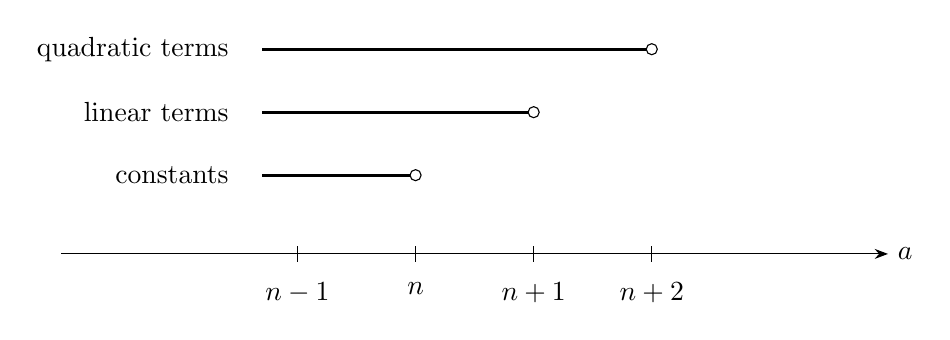
\begin{tikzpicture}[x=1.5cm,y=1cm]
\draw[-{Stealth}] (0,0)--(7,0) node[right] {\(a\)};
\foreach \x/\lab in {2/{n-1},3/{n},4/{n+1},5/{n+2}} {
 \draw (\x,.1)--(\x,-.1) node[below=4pt] {\(\lab\)};}
\node[anchor=east] at (1.5,1) {constants};
\draw[very thick] (1.7,1)--(3,1); \draw[fill=white] (3,1) circle (2pt);
\node[anchor=east] at (1.5,1.8) {linear terms};
\draw[very thick] (1.7,1.8)--(4,1.8); \draw[fill=white] (4,1.8) circle (2pt);
\node[anchor=east] at (1.5,2.6) {quadratic terms};
\draw[very thick] (1.7,2.6)--(5,2.6); \draw[fill=white] (5,2.6) circle (2pt);
\end{tikzpicture}
\end{center}
A term of degree \(k\) is allowed precisely when \(a<k+n\).
\[
a=n:\quad\cI_h=\mathfrak m_0,
\qquad
a=n+1:\quad\cI_h=\mathfrak m_0^2.
\]
\end{frame}

\begin{frame}{Curvature still makes sense}
\[
i\Theta_h=2i\partial\db\varphi.
\]
For singular \(\varphi\), interpret the derivatives as currents.
\[
i\Theta_h\ge\varepsilon\omega
\]
means strict positivity in that sense.
\medskip
\par Psh weights supply positive curvature locally.
\end{frame}

\begin{frame}{The Dolbeault argument we already know}
\begin{columns}[c]
\column{.32\textwidth}
\centering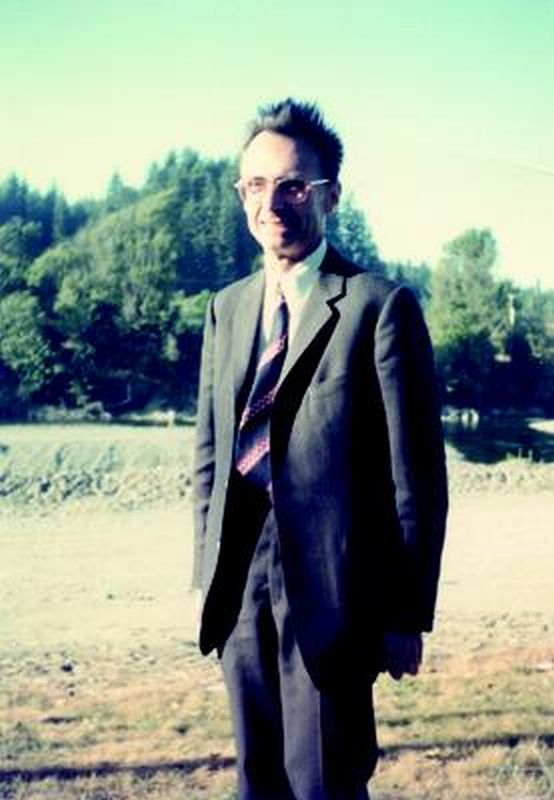
\includegraphics[height=4.6cm]{../assets/Pierre_Dolbeault.jpg}
\column{.65\textwidth}
Local primitives make the complex exact.
\par\bigskip
\par Partitions of unity make its sheaves fine.
\par\bigskip
\par Its global complex computes sheaf cohomology.
\end{columns}
\src{Pierre Dolbeault. The same resolution argument as in our earlier lectures (Daniel).}
\end{frame}

\begin{frame}{The weighted Dolbeault complex}
Use \(B\)-valued forms with
\[
u,\ \db u\in L^2_{\rm loc}(h).
\]
The degree-zero kernel is \(K_X\otimes B\otimes\cI_h\), so the complex begins
\[
0\longrightarrow K_X\otimes B\otimes\cI_h
\longrightarrow\cA_h^{n,0}\xrightarrow{\db}\cA_h^{n,1}
\xrightarrow{\db}\cdots .
\]
The derivative is distributional.
\end{frame}

\begin{frame}{Why this computes cohomology}
\textbf{Local exactness:} the weighted local \(\db\)-lemma gives primitives.
This is an analytic input.
\par\bigskip
\par \textbf{Fineness:} smooth cutoffs preserve the domain, since
\[
\db(\chi u)=\db\chi\wedge u+\chi\,\db u.
\]
\par\bigskip
\par Thus a class is represented by a global closed \(L^2_h\) form \(f\).
\end{frame}

\begin{frame}{Vanishing is now a solvability problem}
\begin{center}
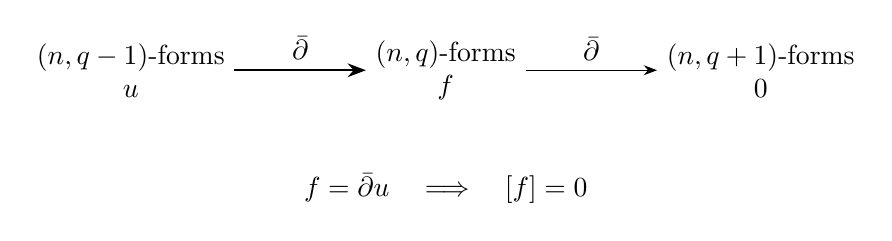
\begin{tikzpicture}[>=Stealth,every node/.style={align=center}]
\node (a) at (-4,0) {\((n,q-1)\)-forms\\\(u\)};
\node (b) at (0,0) {\((n,q)\)-forms\\\(f\)};
\node (c) at (4,0) {\((n,q+1)\)-forms\\\(0\)};
\draw[->,thick] (a)--node[above] {\(\db\)} (b);
\draw[->] (b)--node[above] {\(\db\)} (c);
\node at (0,-1.5) {\(f=\db u\quad\Longrightarrow\quad[f]=0\)};
\end{tikzpicture}
\end{center}
The primitive must satisfy the same \(L^2_h\) condition.
\end{frame}

\begin{frame}{The analytic theorem we use}
Under \(i\Theta_h\ge\varepsilon\omega\), for \(q>0\),
\[
\db f=0,\quad \norm{f}_h<\infty
\quad\Longrightarrow\quad
\db u=f,
\]
with
\[
\boxed{\norm{u}_h^2\le\frac{1}{q\varepsilon}\norm{f}_h^2.}
\]
This is the singular-weight \(L^2\) existence theorem.
Its full analytic proof is an input to this lecture.
\end{frame}

\begin{frame}{The idea behind singular weights}
\begin{columns}[c]
\column{.49\textwidth}
\centering
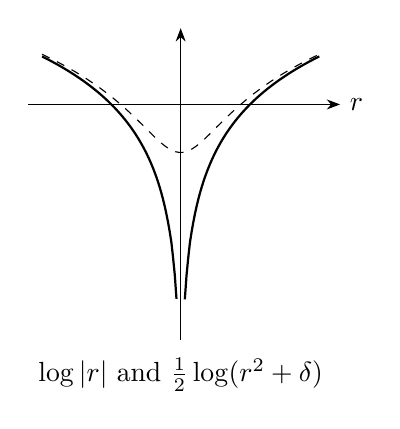
\begin{tikzpicture}[scale=.88,>=Stealth]
\draw[->] (-2.2,0)--(2.3,0) node[right] {\(r\)};
\draw[->] (0,-3.4)--(0,1.1);
\draw[thick,domain=.06:2,samples=80] plot (\x,{ln(\x)});
\draw[thick,domain=-2:-.06,samples=80] plot (\x,{ln(-\x)});
\draw[dashed,domain=-2:2,samples=80] plot (\x,{.5*ln(\x*\x+.25)});
\node at (0,-3.9) {\(\log|r|\) and \(\frac12\log(r^2+\delta)\)};
\end{tikzpicture}
\column{.48\textwidth}
Smooth the local weights.
\par\bigskip
\par Keep a uniform \(L^2\) estimate.
\par\bigskip
\par Take a weak limit of the solutions.
\end{columns}
\src{Local model only. The global theorem also requires control of domains and curvature errors.}
\end{frame}

\begin{frame}{Nadel: the proof}
\begin{enumerate}
\setlength{\itemsep}{14pt}
\item The weighted resolution represents a class by a closed form \(f\).
\item The analytic theorem solves \(\db u=f\) with \(u\in L^2_h\).
\item The class is exact, hence zero.
\end{enumerate}
\[
\boxed{H^q(X,K_X\otimes B\otimes\cI_h)=0\quad(q>0).}
\]
\end{frame}

\begin{frame}{Nadel now fits the embedding mechanism}
Set \(B_N=L^N\otimes K_X^{-1}\). Then
\[
K_X\otimes B_N=L^N.
\]
If \(B_N\) has a strictly positive singular metric with \(\cI_h=I\), Nadel gives
\[
\boxed{H^1(X,L^N\otimes I)=0.}
\]
For the three ideals from the opening, this gives exactly the sections needed for embedding.
\end{frame}

\begin{frame}{Where we stand}
\begin{enumerate}
\setlength{\itemsep}{13pt}
\item We reduced embedding to prescribing values and first derivatives.
\item We reduced those prescriptions to \(H^1\)-vanishing.
\item Nadel supplies that vanishing for multiplier ideals.
\end{enumerate}
\par\bigskip
\textbf{Next step:} put logarithmic poles into a positive metric on \(B_N\), with one exponent \(N\) valid everywhere.
\end{frame}
\end{document}
